\chapter{Der Simulator}

\section{Die grafische Benutzerschnittstelle}

\begin{figure}[htbp]
	\centering
	\fbox{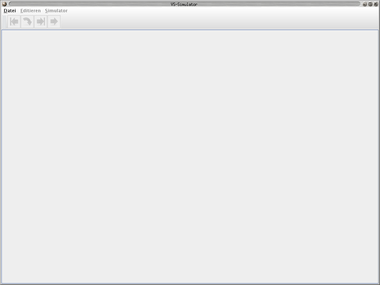
\includegraphics{images/ss-neues-fenster-klein}}
	\caption{Der Simulator nach dem ersten Starten}
	\label{fig:NeuesFenster}

\end{figure}
Der Simulator pr\"{a}sentiert sich nach dem ersten Starten wie in Abbildung \ref{fig:NeuesFenster}. F\"{u}r die Erstellung einer neuen Simulation wird im Men\"{u} ``Datei'' (Abbildung \ref{fig:DateiMenue}) der Punkt ``Neue Simulation'' ausgew\"{a}hlt, wo anschlie�end das Einstellungsfenster f\"{u}r die neu zu erstellende Simulation erscheint.  Auf die einzelnen Optionen wird sp\"{a}ter genauer eingegangen und es werden nun nur die Standardeinstellungen \"{u}bernommen. Die GUI mit einer frischen Simulation sieht dann wie in Abbildung \ref{fig:NeuErstellteSimulation} aus.

\begin{figure}[htbp]
	\centering
	\fbox{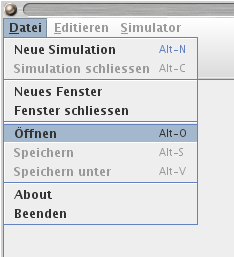
\includegraphics[width=14cm]{images/ss-datei-menu}}
	\caption{Datei-Men\"{u}}
	\label{fig:DateiMenue}
\end{figure}

\subsection{Die Men\"{u}zeile}

Im Datei-Men\"{u} (Abbildung \ref{fig:DateiMenue}) lassen sich neue Simulationen erstellen oder die aktuell ge\"{o}ffnete Simulation schliessen. Neue Simulationen \"{o}ffnen sich standardm\"{a}�ig in einem neuen Tab. Es k\"{o}nnen allerdings auch neue Simulationsfenster, die wiederrum eigene Tabs besitzen, ge\"{o}ffnet oder geschlossen werden. In jedem Tab befindet sich eine von den Anderen vollst\"{a}ndig unabh\"{a}ngige Simulation. Es k\"{o}nnen somit beliebig viele Simulationen parallel ausgef\"{u}hrt werden. Die Men\"{u}eintr\"{a}ge ``\"{O}ffnen'', ``Speichern'' und ``Speichern unter'' dienen f\"{u}r das Laden und Speichern von Simulationen. 

\begin{figure}[htbp]
	\centering
	\fbox{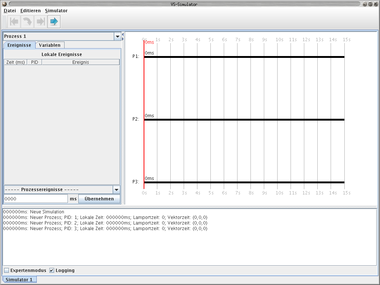
\includegraphics{images/ss-neue-simulation-klein}}
	\caption{Eine neuerstellte Simulation}
	\label{fig:NeuErstellteSimulation}
\end{figure}

\"{U}ber das Editieren-Men\"{u} gelangt man zu den Simulationseinstellungen, worauf sp\"{a}ter genauer eingegangen wird. Es werden in diesem Men\"{u} auch alle beteiligten Prozesse zum Editieren aufgelistet. Das Simulator-Men\"{u} bietet die selben Optionen wie die Toolbar, welche im n\"{a}chsten Teilkapitel beschrieben wird.

Einige Men\"{u}s sind erst erreichbar, wenn im aktuellen Fenster bereits eine Simulation erstellt oder geladen wurde.

\subsection{Die Toolbar}

Oben links im Simulator befindet sich die Toolbar (Abbildung \ref{fig:Toolbar}). Die Toolbar enth\"{a}lt die Funktionen, die vom Benutzer am h\"{a}ufigsten verwendet werden.

\begin{figure}[htbp]
	\centering
	\fbox{
\includegraphics[width=5cm]{images/ss-neue-simulation-toolbar}}
	\caption{Die Men\"{u}zeile inklusive Toolbar}
	\label{fig:Toolbar}
\end{figure}

Die Toolbar bietet vier verschiedene Funktionalit\"{a}ten an:

\begin{itemize}
	%\setlength{\itemsep}{-1mm}
	\item Starten der Simulation; kann nur bet\"{a}tigt werden, wenn die Simulation derzeit nicht l\"{a}uft.
	\item Pausieren der Simulation, kann nur bet\"{a}tigt werden, wenn die Simulation derzeit l\"{a}uft.
	\item Wiederholen der Simulation, kann nicht bet\"{a}tigt werden, wenn die Simulation noch nicht gestartet wurde. 
	\item Zur\"{u}cksetzen der Simulation, kann nur bet\"{a}tigt werden, wenn die Simulation pausiert wurde oder wenn die Simulation abgelaufen ist.
\end{itemize}

Die Toolbar l\"{a}sst sich auch nach Belieben repositionieren (z.B. links, rechts oder unten des Simulatorfensters). Hierf\"{u}r muss per ``Drag-n-Drop'' die ``raue Fl\"{a}che'' zur Zielposition gezogen werden.

\subsection{Die Visualisierung}

\begin{figure}[htbp]
	\centering
	\fbox{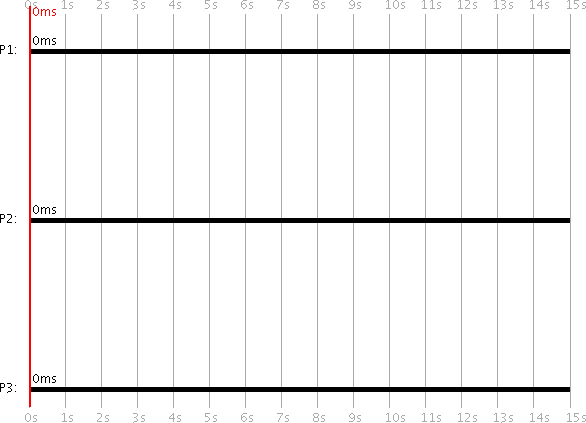
\includegraphics[width=14cm]{images/ss-visualisierung}}
	\caption{Visualisierung einer noch nicht gestarteten Simulation}
	\label{fig:Visualisierung}
\end{figure}

Mittig rechts (Abbildung \ref{fig:NeuErstellteSimulation}) befindet sich die grafische Repr\"{a}sentation der Simulation. Die X-Achse repr\"{a}sentiert die Zeit in Millisekunden. Die aktuelle Simulation endet nach genau 15 Sekunden. In Abbildung \ref{fig:Visualisierung} sind 3 Prozesse (mit den PIDs 1, 2 und 3) dargestellt, die jeweils einen eigenen horizontalen schwarzen Balken besitzen. Auf diesen Prozessbalken kann man die jeweilige lokale Prozesszeit ablesen. Die vertikale rote Linie stellt die globale Zeit dar. 

Die Prozessbalken dienen auch f\"{u}r Start- und Zielpunkte von Nachrichten. Wenn beispielsweise Prozess 1 eine Nachricht zum Prozess 2 verschickt, so wird eine Linie vom einen Prozessbalken zum Anderen gezeichnet. Nachrichten, die ein Prozess an sich selbst schickt, werden nicht visualisiert.

Mit einem Linksklick auf einen Prozessbalken ist es ebenso m\"{o}glich einen Prozess zu editieren. Dies muss also nicht zwingend \"{u}ber das Simulator-Men\"{u} geschehen. Ein Rechtsklick hingegen \"{o}ffnet ein Popup-Fenster mit weiteren Auswahlm\"{o}glichkeiten (Abbildung \ref{fig:RechtsklickProzessbalken}). Ein Prozess kann \"{u}ber das Popup-Men\"{u} nur dann abst\"{u}rzen oder wiederbelebt werden, wenn die Simulation aktuell l\"{a}uft.

\begin{figure}[htbp]
	\centering
	\fbox{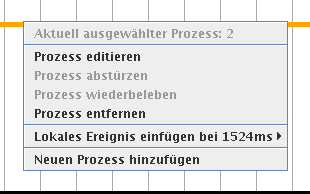
\includegraphics[width=8.8cm]{images/ss-rechtsklick-prozessbalken}}
	\caption{Rechtsklick auf einen Prozessbalken}
	\label{fig:RechtsklickProzessbalken}
\end{figure}

Generell kann die Anzahl der Prozesse nach belieben variieren. Die Dauer der Simulation betr\"{a}gt mindestens 5 -und maximal 120 Sekunden. Die Simulation endet erst, wenn die globale Zeit 15 Sekunden erreicht hat, und nicht, wenn eine lokale Prozesszeit die 15 Sekunden erreicht.

\subsubsection{Farbliche Differenzierung}

F\"{u}r Visualisierung einer Simulation spielen Farben eine gro�e Rolle. Standardm\"{a}�ig werden die Prozesse (Prozessbalken) und Nachrichten mit den Farben wie in Tabelle \ref{tb:Farben} aufgelistet dargestellt. Dies sind lediglich die Standarfarben, welche man \"{u}ber die Einstellungen neudefinieren kann.

\begin{table}
	\fbox{
	\begin{tabular}{c|l}
		\textbf{Prozessfarbe} & \textbf{Bedeutung} \\
		\hline 
		 	Schwarz & Simulation l\"{a}uft derzeit nicht (z.B. noch nicht gestartet, abgelaufen oder\\
				& pausiert)\\
		 	Orange & Die Maus befindet sich \"{u}ber den Prozessbalken\\
		 	Rot & Der Prozess ist abgest\"{u}rzt\\
			& \\
		\textbf{Nachrichtfarbe} & \textbf{Bedeutung} \\
		\hline 
		 	Gr\"{u}n & Die Nachricht ist noch unterwegs hat das Ziel noch nicht erreicht\\
		 	Blau & Die Nachricht hat das Ziel erfolgreich erreicht\\
		 	Rot & Die Nachricht ging verloren (entweder weil der Zielprozess abgest\"{u}rzt ist\\
				& oder weil sie unterwegs verloren ging)\\

	\end{tabular}\\
	}
	\caption{Farbliche Differenzierung von Prozessen und Nachrichten}
	\label{tb:Farben}
\end{table}

\subsection{Die Sidebar}

Mithilfe der Sidebar (mittig links, Abbildung \ref{fig:NeuErstellteSimulation}) lassen sich Ereignisse bestimmter Prozesse verwalten. Ganz oben in Abbildung \ref{fig:Sidebar} ist der zu verwaltende Prozess selektiert (hier mit der PID 1). In dieser Prozessauswahl gibt es auch die M\"{o}glichkeit ``Alle Prozesse'' auszuw\"{a}hlen, womit die Ereignisse aller Prozesse gleichzeitig verwaltet werden k\"{o}nnen. Unter ``Lokale Ereignisse'' versteht man die Ereignisse, die auftreten, wenn die zum jeweiligen Prozess lokale Prozesszeit eingetreten ist. Die darunterliegende Ereignistabelle listet alle programmierten Ereignisse (hier noch keine vorhanden) mitsamt Eintrittszeit sowie PID auf.

\begin{figure}[htbp]
	\centering
	\fbox{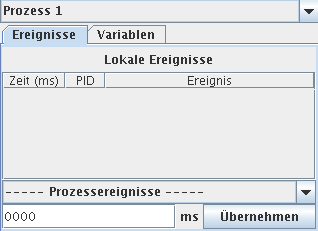
\includegraphics[width=9cm]{images/ss-sidebar}}
	\caption{Die Sidebar mit noch keinen programmierten Ereignissen}
	\label{fig:Sidebar}
\end{figure}

F\"{u}r die Erstellung eines neuen Ereignisses kann man entweder mit einem Rechtsklick auf einen Prozessbalken (Abbildung \ref{fig:RechtsklickProzessbalken}) klicken, oder unterhalb der Ereignistabelle ein Ereignis ausw\"{a}hlen (Abbildung \ref{fig:Ereignisauswahl}), im darunterliegendem Textfeld die Zeit eintragen und auf ``\"{U}bernehmen'' klicken. Beispielsweise wurden auf Abbildung \ref{fig:SidebarMitEreignissen} drei Ereignisse hinzugef\"{u}gt: Absturz nach 123ms, Wiederbelebung nach 321ms und erneuerter Absturz nach 3000ms des Prozesses mit der ID 1. 

\begin{figure}[htbp]
	\centering
	\fbox{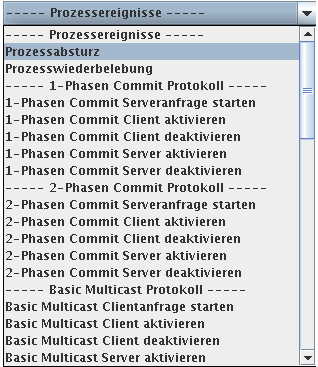
\includegraphics[width=9cm]{images/ss-ereignisauswahl}}
	\caption{Die Ereignisauswahl via Sidebar}
	\label{fig:Ereignisauswahl}
\end{figure}

Mit einem Rechtsklick auf den Ereigniseditor lassen sich alle selektierten Ereignisse entweder kopieren oder l\"{o}schen. Die Spalten f\"{u}r die Zeit und der PID lassen sich nachtr\"{a}glich editieren. Somit besteht eine komfortable M\"{o}glichkeit bereits programmierte Ereignisse auf eine andere Zeit zu verschieben oder einem anderen Prozess zuzuweisen.

In der Sidebar gibt es neben dem Ereignis-Tab einen weiteren Tab ``Variablen''. Dort k\"{o}nnen alle Variablen des aktuell ausgew\"{a}hlten Prozesses editiert werden. Mehr dazu aber sp\"{a}ter. 

\begin{figure}[htbp]
	\centering
	\fbox{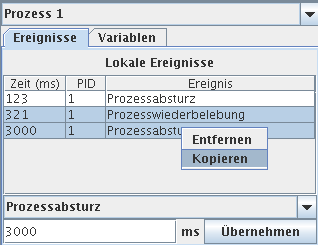
\includegraphics[width=9cm]{images/ss-sidebar-mit-ereignissen}}
	\caption{Der Ereigniseditor mit 3 programmierten Ereignissen}
	\label{fig:SidebarMitEreignissen}
\end{figure}

\subsection{Das Loggfenster}

Das Loggfenster (Abbildung \ref{fig:NeuErstellteSimulation}, unten) protokolliert  in chronologischer Reihenfolge alle eingetroffenen Ereignisse. Auf Abbildung \ref{fig:Loggfenster} sieht man das Loggfenster nach Erstellung unserer Simulation, an welcher 3 Prozesse beteiligt sind. Am Anfang eines Loggeintrages wird stets die globale Zeit in Millisekunden protokolliert. Bei jedem Prozess wird ebenso seine lokale Zeit sowie die Lamport- und die Vektor-Zeitstempel aufgef\"{u}hrt. Letztere werden sp\"{a}ter genauer behandelt. 

\begin{figure}[htbp]
	\centering
	\fbox{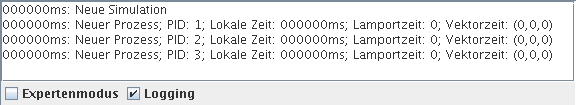
\includegraphics[width=16.5cm]{images/ss-loggfenster}}
	\caption{Das Loggfenster}
	\label{fig:Loggfenster}
\end{figure}

Mit dem Deaktivieren der Checkbox ``Logging'' l\"{a}�t sich das direkte Loggen von Nachrichten tempor\"{a}r ausstellen. Ohne aktivierter Checkbox erscheinen keine neuen Nachrichten mehr im Loggfenster. Nach Reaktivieren der Checkbox werden alle ausgelassenen Nachrichten nachtr\"{a}glich in das Fenster geschrieben. Eine Deaktivierung des Loggings kann zu verbessertem Leistungsverhalten des Simulators f\"{u}hren (z.B. kein Rucklen; ist vom verwendeten Computer, auf dem der Simulator l\"{a}uft, abh\"{a}ngig). 

\"{U}ber die Checkbox ``Expertenmodus'' wird der Expertenmodus aktiviert beziehungsweise deaktiviert. 

\subsection{Der Expertenmodus}
 lsdkfjds lfjds flsjfsljsd flsdjf sldkfjsdlfkj 
 lsdkfjds lfjds flsjfsljsd flsdjf sldkfjsdlfkj 
 lsdkfjds lfjds flsjfsljsd flsdjf sldkfjsdlfkj 
 lsdkfjds lfjds flsjfsljsd flsdjf sldkfjsdlfkj 
 lsdkfjds lfjds flsjfsljsd flsdjf sldkfjsdlfkj 
 lsdkfjds lfjds flsjfsljsd flsdjf sldkfjsdlfkj 
 lsdkfjds lfjds flsjfsljsd flsdjf sldkfjsdlfkj 
 lsdkfjds lfjds flsjfsljsd flsdjf sldkfjsdlfkj 
 lsdkfjds lfjds flsjfsljsd flsdjf sldkfjsdlfkj 
 lsdkfjds lfjds flsjfsljsd flsdjf sldkfjsdlfkj 
 lsdkfjds lfjds flsjfsljsd flsdjf sldkfjsdlfkj 
 lsdkfjds lfjds flsjfsljsd flsdjf sldkfjsdlfkj 
 lsdkfjds lfjds flsjfsljsd flsdjf sldkfjsdlfkj 
 lsdkfjds lfjds flsjfsljsd flsdjf sldkfjsdlfkj 
 lsdkfjds lfjds flsjfsljsd flsdjf sldkfjsdlfkj 
 lsdkfjds lfjds flsjfsljsd flsdjf sldkfjsdlfkj 
 lsdkfjds lfjds flsjfsljsd flsdjf sldkfjsdlfkj 
 lsdkfjds lfjds flsjfsljsd flsdjf sldkfjsdlfkj 
 lsdkfjds lfjds flsjfsljsd flsdjf sldkfjsdlfkj 
 lsdkfjds lfjds flsjfsljsd flsdjf sldkfjsdlfkj 
 lsdkfjds lfjds flsjfsljsd flsdjf sldkfjsdlfkj 
 lsdkfjds lfjds flsjfsljsd flsdjf sldkfjsdlfkj 
 lsdkfjds lfjds flsjfsljsd flsdjf sldkfjsdlfkj 
 lsdkfjds lfjds flsjfsljsd flsdjf sldkfjsdlfkj 
 lsdkfjds lfjds flsjfsljsd flsdjf sldkfjsdlfkj 
 lsdkfjds lfjds flsjfsljsd flsdjf sldkfjsdlfkj 
 lsdkfjds lfjds flsjfsljsd flsdjf sldkfjsdlfkj 
 lsdkfjds lfjds flsjfsljsd flsdjf sldkfjsdlfkj 
 lsdkfjds lfjds flsjfsljsd flsdjf sldkfjsdlfkj 
 lsdkfjds lfjds flsjfsljsd flsdjf sldkfjsdlfkj 
 lsdkfjds lfjds flsjfsljsd flsdjf sldkfjsdlfkj 
 lsdkfjds lfjds flsjfsljsd flsdjf sldkfjsdlfkj 
 lsdkfjds lfjds flsjfsljsd flsdjf sldkfjsdlfkj 
 lsdkfjds lfjds flsjfsljsd flsdjf sldkfjsdlfkj 
 lsdkfjds lfjds flsjfsljsd flsdjf sldkfjsdlfkj 
 lsdkfjds lfjds flsjfsljsd flsdjf sldkfjsdlfkj 
 lsdkfjds lfjds flsjfsljsd flsdjf sldkfjsdlfkj 
 lsdkfjds lfjds flsjfsljsd flsdjf sldkfjsdlfkj 
 lsdkfjds lfjds flsjfsljsd flsdjf sldkfjsdlfkj 
 lsdkfjds lfjds flsjfsljsd flsdjf sldkfjsdlfkj 
 lsdkfjds lfjds flsjfsljsd flsdjf sldkfjsdlfkj 
 lsdkfjds lfjds flsjfsljsd flsdjf sldkfjsdlfkj 
 lsdkfjds lfjds flsjfsljsd flsdjf sldkfjsdlfkj 
 lsdkfjds lfjds flsjfsljsd flsdjf sldkfjsdlfkj 
 lsdkfjds lfjds flsjfsljsd flsdjf sldkfjsdlfkj 
 lsdkfjds lfjds flsjfsljsd flsdjf sldkfjsdlfkj 
 lsdkfjds lfjds flsjfsljsd flsdjf sldkfjsdlfkj 
 lsdkfjds lfjds flsjfsljsd flsdjf sldkfjsdlfkj 
 lsdkfjds lfjds flsjfsljsd flsdjf sldkfjsdlfkj 
 lsdkfjds lfjds flsjfsljsd flsdjf sldkfjsdlfkj 
 lsdkfjds lfjds flsjfsljsd flsdjf sldkfjsdlfkj 
 lsdkfjds lfjds flsjfsljsd flsdjf sldkfjsdlfkj 
 lsdkfjds lfjds flsjfsljsd flsdjf sldkfjsdlfkj 
 lsdkfjds lfjds flsjfsljsd flsdjf sldkfjsdlfkj 
 lsdkfjds lfjds flsjfsljsd flsdjf sldkfjsdlfkj 
 lsdkfjds lfjds flsjfsljsd flsdjf sldkfjsdlfkj 
 lsdkfjds lfjds flsjfsljsd flsdjf sldkfjsdlfkj 
 lsdkfjds lfjds flsjfsljsd flsdjf sldkfjsdlfkj 
 lsdkfjds lfjds flsjfsljsd flsdjf sldkfjsdlfkj 
 lsdkfjds lfjds flsjfsljsd flsdjf sldkfjsdlfkj 
 lsdkfjds lfjds flsjfsljsd flsdjf sldkfjsdlfkj 
 lsdkfjds lfjds flsjfsljsd flsdjf sldkfjsdlfkj 
 lsdkfjds lfjds flsjfsljsd flsdjf sldkfjsdlfkj 
 lsdkfjds lfjds flsjfsljsd flsdjf sldkfjsdlfkj 
 lsdkfjds lfjds flsjfsljsd flsdjf sldkfjsdlfkj 
 lsdkfjds lfjds flsjfsljsd flsdjf sldkfjsdlfkj 
 lsdkfjds lfjds flsjfsljsd flsdjf sldkfjsdlfkj 
 lsdkfjds lfjds flsjfsljsd flsdjf sldkfjsdlfkj 
 lsdkfjds lfjds flsjfsljsd flsdjf sldkfjsdlfkj 
 lsdkfjds lfjds flsjfsljsd flsdjf sldkfjsdlfkj 
 lsdkfjds lfjds flsjfsljsd flsdjf sldkfjsdlfkj 
 lsdkfjds lfjds flsjfsljsd flsdjf sldkfjsdlfkj 
 lsdkfjds lfjds flsjfsljsd flsdjf sldkfjsdlfkj 
 lsdkfjds lfjds flsjfsljsd flsdjf sldkfjsdlfkj 
 lsdkfjds lfjds flsjfsljsd flsdjf sldkfjsdlfkj 
 lsdkfjds lfjds flsjfsljsd flsdjf sldkfjsdlfkj 
 lsdkfjds lfjds flsjfsljsd flsdjf sldkfjsdlfkj 
 lsdkfjds lfjds flsjfsljsd flsdjf sldkfjsdlfkj 
 lsdkfjds lfjds flsjfsljsd flsdjf sldkfjsdlfkj 
 lsdkfjds lfjds flsjfsljsd flsdjf sldkfjsdlfkj 
 lsdkfjds lfjds flsjfsljsd flsdjf sldkfjsdlfkj 
 lsdkfjds lfjds flsjfsljsd flsdjf sldkfjsdlfkj 
 lsdkfjds lfjds flsjfsljsd flsdjf sldkfjsdlfkj 
 lsdkfjds lfjds flsjfsljsd flsdjf sldkfjsdlfkj 
 lsdkfjds lfjds flsjfsljsd flsdjf sldkfjsdlfkj 
 lsdkfjds lfjds flsjfsljsd flsdjf sldkfjsdlfkj 
 lsdkfjds lfjds flsjfsljsd flsdjf sldkfjsdlfkj 
 lsdkfjds lfjds flsjfsljsd flsdjf sldkfjsdlfkj 
 lsdkfjds lfjds flsjfsljsd flsdjf sldkfjsdlfkj 
 lsdkfjds lfjds flsjfsljsd flsdjf sldkfjsdlfkj 
 lsdkfjds lfjds flsjfsljsd flsdjf sldkfjsdlfkj 
 lsdkfjds lfjds flsjfsljsd flsdjf sldkfjsdlfkj 
 lsdkfjds lfjds flsjfsljsd flsdjf sldkfjsdlfkj 
 lsdkfjds lfjds flsjfsljsd flsdjf sldkfjsdlfkj 
 lsdkfjds lfjds flsjfsljsd flsdjf sldkfjsdlfkj 
 lsdkfjds lfjds flsjfsljsd flsdjf sldkfjsdlfkj 
 lsdkfjds lfjds flsjfsljsd flsdjf sldkfjsdlfkj 
 lsdkfjds lfjds flsjfsljsd flsdjf sldkfjsdlfkj 
 lsdkfjds lfjds flsjfsljsd flsdjf sldkfjsdlfkj 
 lsdkfjds lfjds flsjfsljsd flsdjf sldkfjsdlfkj 
 lsdkfjds lfjds flsjfsljsd flsdjf sldkfjsdlfkj 
 lsdkfjds lfjds flsjfsljsd flsdjf sldkfjsdlfkj 
 lsdkfjds lfjds flsjfsljsd flsdjf sldkfjsdlfkj 
 lsdkfjds lfjds flsjfsljsd flsdjf sldkfjsdlfkj 
 lsdkfjds lfjds flsjfsljsd flsdjf sldkfjsdlfkj 
 lsdkfjds lfjds flsjfsljsd flsdjf sldkfjsdlfkj 
 lsdkfjds lfjds flsjfsljsd flsdjf sldkfjsdlfkj 
 lsdkfjds lfjds flsjfsljsd flsdjf sldkfjsdlfkj 
 lsdkfjds lfjds flsjfsljsd flsdjf sldkfjsdlfkj 
 lsdkfjds lfjds flsjfsljsd flsdjf sldkfjsdlfkj 
 lsdkfjds lfjds flsjfsljsd flsdjf sldkfjsdlfkj 
 lsdkfjds lfjds flsjfsljsd flsdjf sldkfjsdlfkj 
 lsdkfjds lfjds flsjfsljsd flsdjf sldkfjsdlfkj 
 lsdkfjds lfjds flsjfsljsd flsdjf sldkfjsdlfkj 
 lsdkfjds lfjds flsjfsljsd flsdjf sldkfjsdlfkj 
 lsdkfjds lfjds flsjfsljsd flsdjf sldkfjsdlfkj 
 lsdkfjds lfjds flsjfsljsd flsdjf sldkfjsdlfkj 
 lsdkfjds lfjds flsjfsljsd flsdjf sldkfjsdlfkj 
 lsdkfjds lfjds flsjfsljsd flsdjf sldkfjsdlfkj 
 lsdkfjds lfjds flsjfsljsd flsdjf sldkfjsdlfkj 
 lsdkfjds lfjds flsjfsljsd flsdjf sldkfjsdlfkj 
 lsdkfjds lfjds flsjfsljsd flsdjf sldkfjsdlfkj 
 lsdkfjds lfjds flsjfsljsd flsdjf sldkfjsdlfkj 
 lsdkfjds lfjds flsjfsljsd flsdjf sldkfjsdlfkj 
 lsdkfjds lfjds flsjfsljsd flsdjf sldkfjsdlfkj 
 lsdkfjds lfjds flsjfsljsd flsdjf sldkfjsdlfkj 
 lsdkfjds lfjds flsjfsljsd flsdjf sldkfjsdlfkj 
 lsdkfjds lfjds flsjfsljsd flsdjf sldkfjsdlfkj 
 lsdkfjds lfjds flsjfsljsd flsdjf sldkfjsdlfkj 
 lsdkfjds lfjds flsjfsljsd flsdjf sldkfjsdlfkj 
 lsdkfjds lfjds flsjfsljsd flsdjf sldkfjsdlfkj 
 lsdkfjds lfjds flsjfsljsd flsdjf sldkfjsdlfkj 
 lsdkfjds lfjds flsjfsljsd flsdjf sldkfjsdlfkj 
 lsdkfjds lfjds flsjfsljsd flsdjf sldkfjsdlfkj 
 lsdkfjds lfjds flsjfsljsd flsdjf sldkfjsdlfkj 
 lsdkfjds lfjds flsjfsljsd flsdjf sldkfjsdlfkj 
 lsdkfjds lfjds flsjfsljsd flsdjf sldkfjsdlfkj 
 lsdkfjds lfjds flsjfsljsd flsdjf sldkfjsdlfkj 
 lsdkfjds lfjds flsjfsljsd flsdjf sldkfjsdlfkj 
 lsdkfjds lfjds flsjfsljsd flsdjf sldkfjsdlfkj 
 lsdkfjds lfjds flsjfsljsd flsdjf sldkfjsdlfkj 
 lsdkfjds lfjds flsjfsljsd flsdjf sldkfjsdlfkj 
 lsdkfjds lfjds flsjfsljsd flsdjf sldkfjsdlfkj 
 lsdkfjds lfjds flsjfsljsd flsdjf sldkfjsdlfkj 
 lsdkfjds lfjds flsjfsljsd flsdjf sldkfjsdlfkj 
 lsdkfjds lfjds flsjfsljsd flsdjf sldkfjsdlfkj 
 lsdkfjds lfjds flsjfsljsd flsdjf sldkfjsdlfkj 
 lsdkfjds lfjds flsjfsljsd flsdjf sldkfjsdlfkj 
 lsdkfjds lfjds flsjfsljsd flsdjf sldkfjsdlfkj 
 lsdkfjds lfjds flsjfsljsd flsdjf sldkfjsdlfkj 
 lsdkfjds lfjds flsjfsljsd flsdjf sldkfjsdlfkj 
 lsdkfjds lfjds flsjfsljsd flsdjf sldkfjsdlfkj 
 lsdkfjds lfjds flsjfsljsd flsdjf sldkfjsdlfkj 
 lsdkfjds lfjds flsjfsljsd flsdjf sldkfjsdlfkj 
 lsdkfjds lfjds flsjfsljsd flsdjf sldkfjsdlfkj 
 lsdkfjds lfjds flsjfsljsd flsdjf sldkfjsdlfkj 
 lsdkfjds lfjds flsjfsljsd flsdjf sldkfjsdlfkj 
 lsdkfjds lfjds flsjfsljsd flsdjf sldkfjsdlfkj 
 lsdkfjds lfjds flsjfsljsd flsdjf sldkfjsdlfkj 
 lsdkfjds lfjds flsjfsljsd flsdjf sldkfjsdlfkj 
 lsdkfjds lfjds flsjfsljsd flsdjf sldkfjsdlfkj 
 lsdkfjds lfjds flsjfsljsd flsdjf sldkfjsdlfkj 


\subsubsection{Lamport- und Vektorzeit}

\subsubsection{Loggfilter}

\subsubsection{Lokale und globale Ereignisse}

\section{Ereignisse}

\subsection{Prozessabsturz}

\subsection{Prozesswiederbelebung}

\subsection{Aktivierung und Deaktivierung von Protokollen}

\subsection{Weitere Protokollereignisse}

\section{Protokolle}

\subsection{Beispiel (Dummy) Protokoll}

\subsection{Das Ping-Pong Protokoll}

\subsection{Das Broadcast-Sturm Protokoll}

\subsection{Das Protokoll zur internen Synchronisierung in einem synchronen System}

\subsection{Christians Methode zur externen Synchronisierung}

\subsection{Berkeley Algorithmus zur internen Synchronisation}

\subsection{Das Ein-Phasen Commit Protokoll}

\subsection{Das Zwei-Phasen Commit Protokoll}

\subsection{Der ungen\"{u}gende (Basic) Multicast}

\subsection{Der zuverl\"{a}ssige (Reliable) Multicast}

\section{Zeitformate}

\subsection{``Normale Zeit''}

\subsection{Die Logische Uhr von Lamport}

\subsection{Die Vektor-Zeitstempel}

\section{Einstellungen}

\subsection{Simulationseinstellungen}

\subsection{Prozesseinstellungen}

\subsection{Protokolleinstellungen}

TODO: Farben der Prozessbalken, Farben der Nachrichten
